\documentclass{standalone}
\usepackage{tikz}

\begin{document}
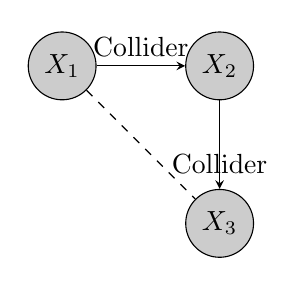
\begin{tikzpicture}[node distance=2cm]
    % Nodes
    \node (X1) [circle, draw, fill=black!20] {$X_1$};
    \node (X2) [circle, draw, fill=black!20, right of=X1] {$X_2$};
    \node (X3) [circle, draw, fill=black!20, below of=X2] {$X_3$};

    % Edges
    \draw[-stealth] (X1) -- node[above] {Collider} (X2);
    \draw[-stealth] (X2) -- node[below] {Collider} (X3);

    % Collider edges
    \draw[dashed] (X1) -- node[left] {} (X3);
\end{tikzpicture}
\end{document}